\begin{figure}[!htbp]
 \centering
    \begin{subfigure}[b]{0.5\textwidth}
        \centering
    	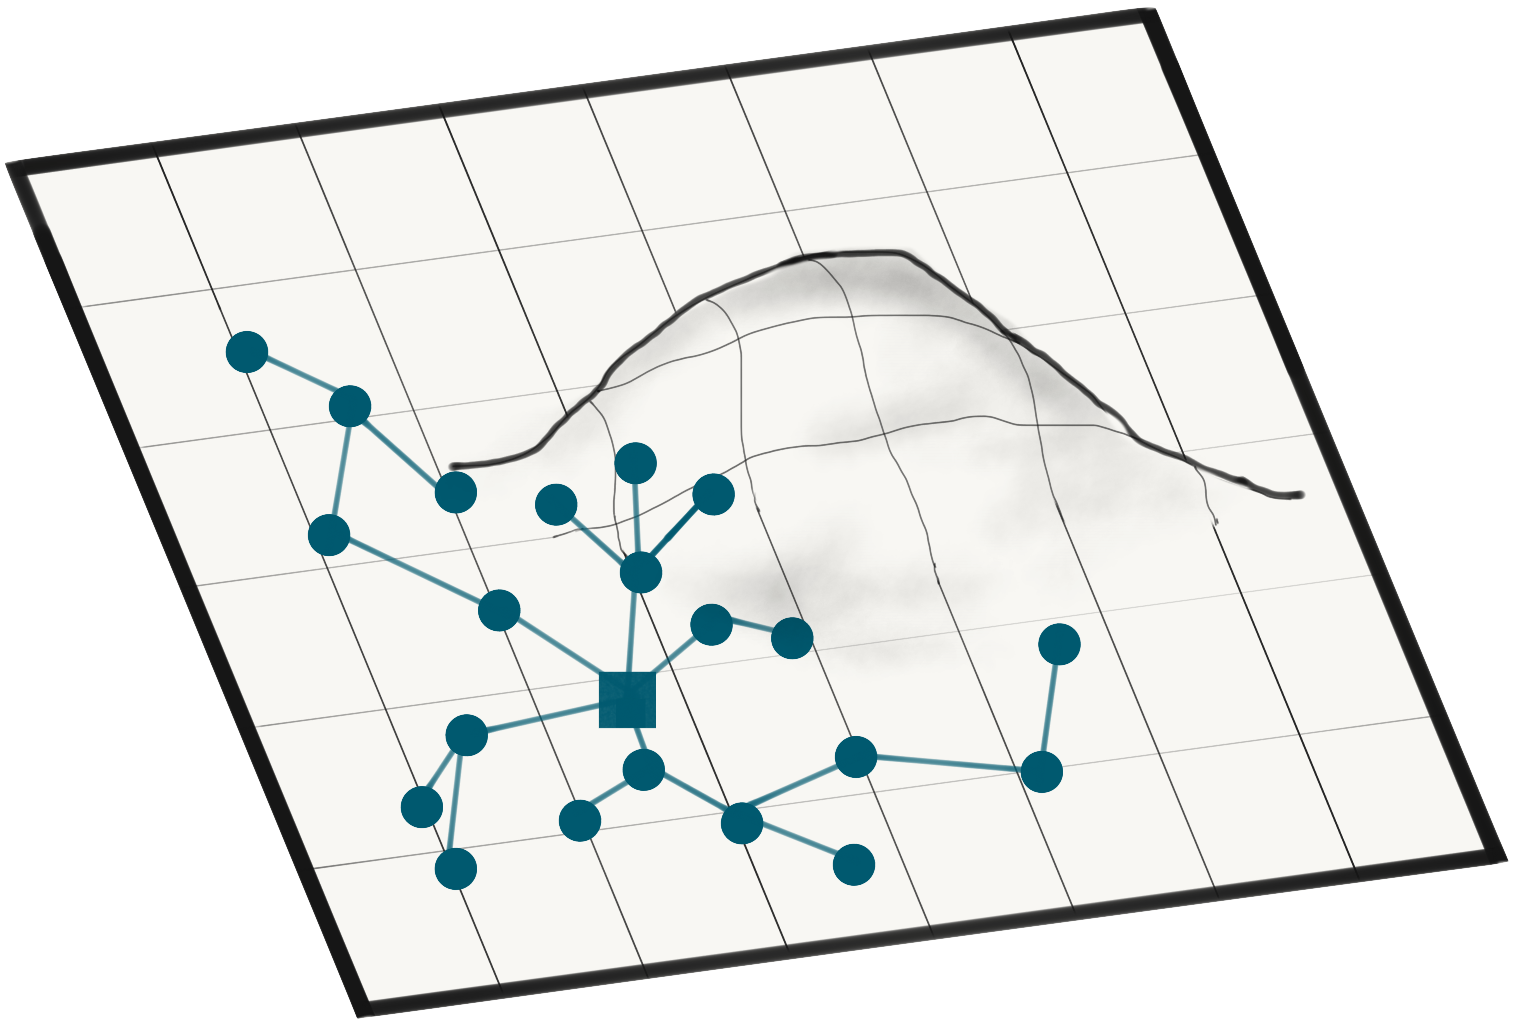
\includegraphics[width=\textwidth]{img/slow_cooling.png}
        \caption{slow cooling rate}
        \label{subfig:slow_cooling}
    \end{subfigure}%
    \hfill
    \begin{subfigure}[b]{0.5\textwidth}
        \centering
        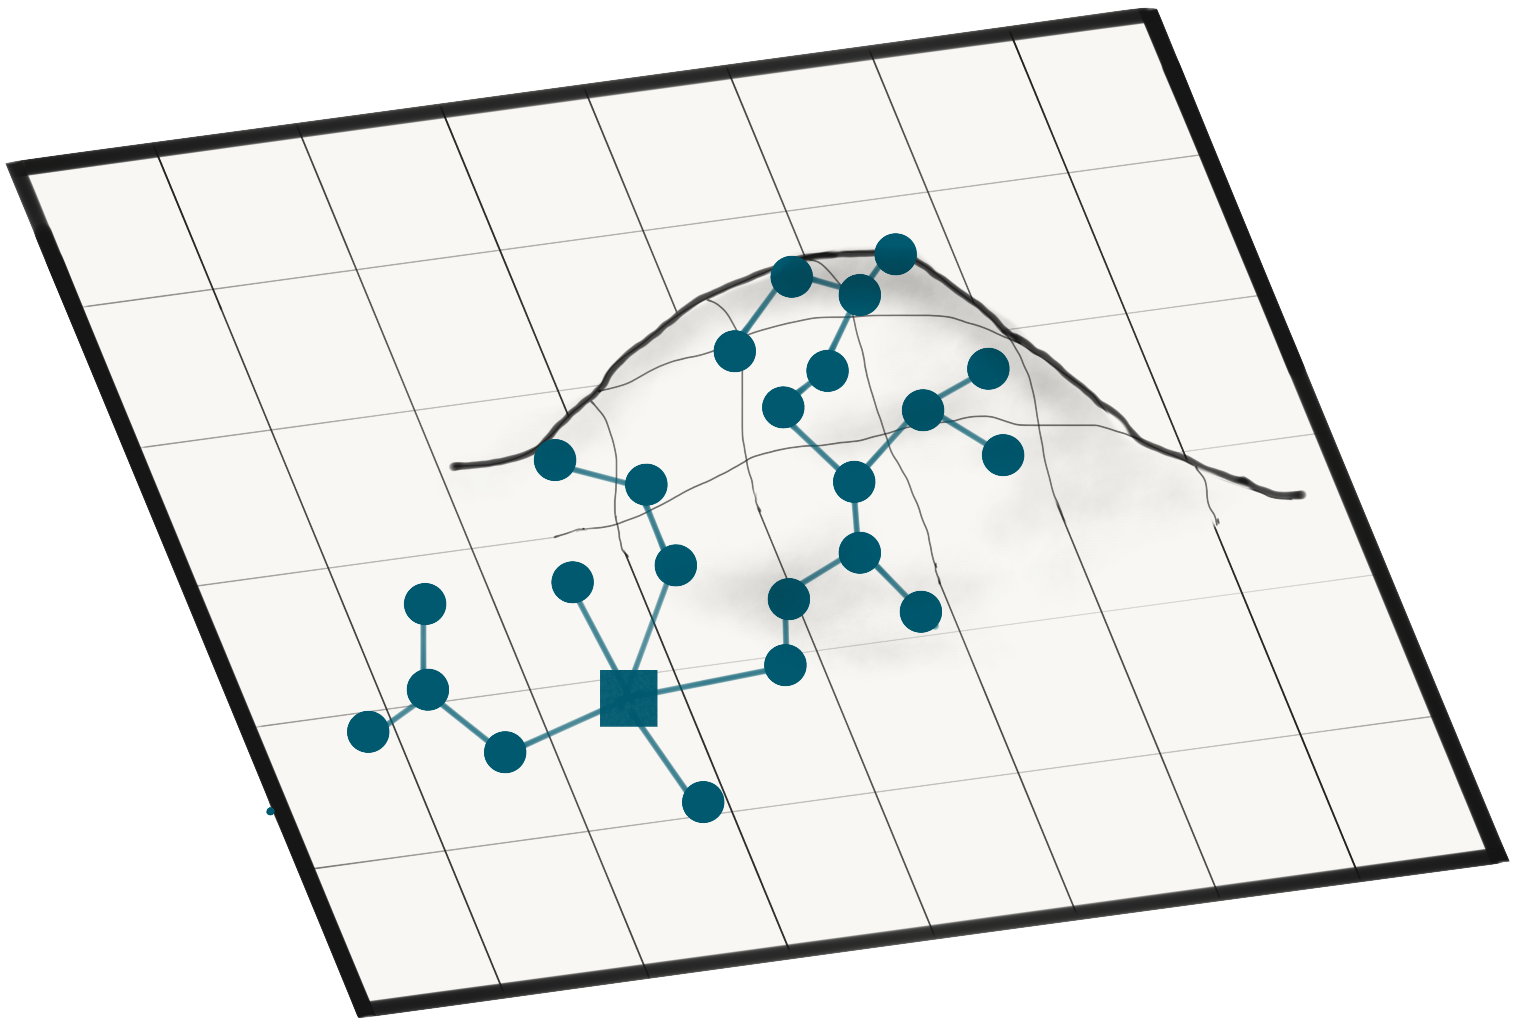
\includegraphics[width=\textwidth]{img/medium_cooling.png}
        \caption{medium cooling rate}
        \label{subfig:slow_cooling}
    \end{subfigure}
    \hfill
    \begin{subfigure}[b]{0.5\textwidth}
        \centering
        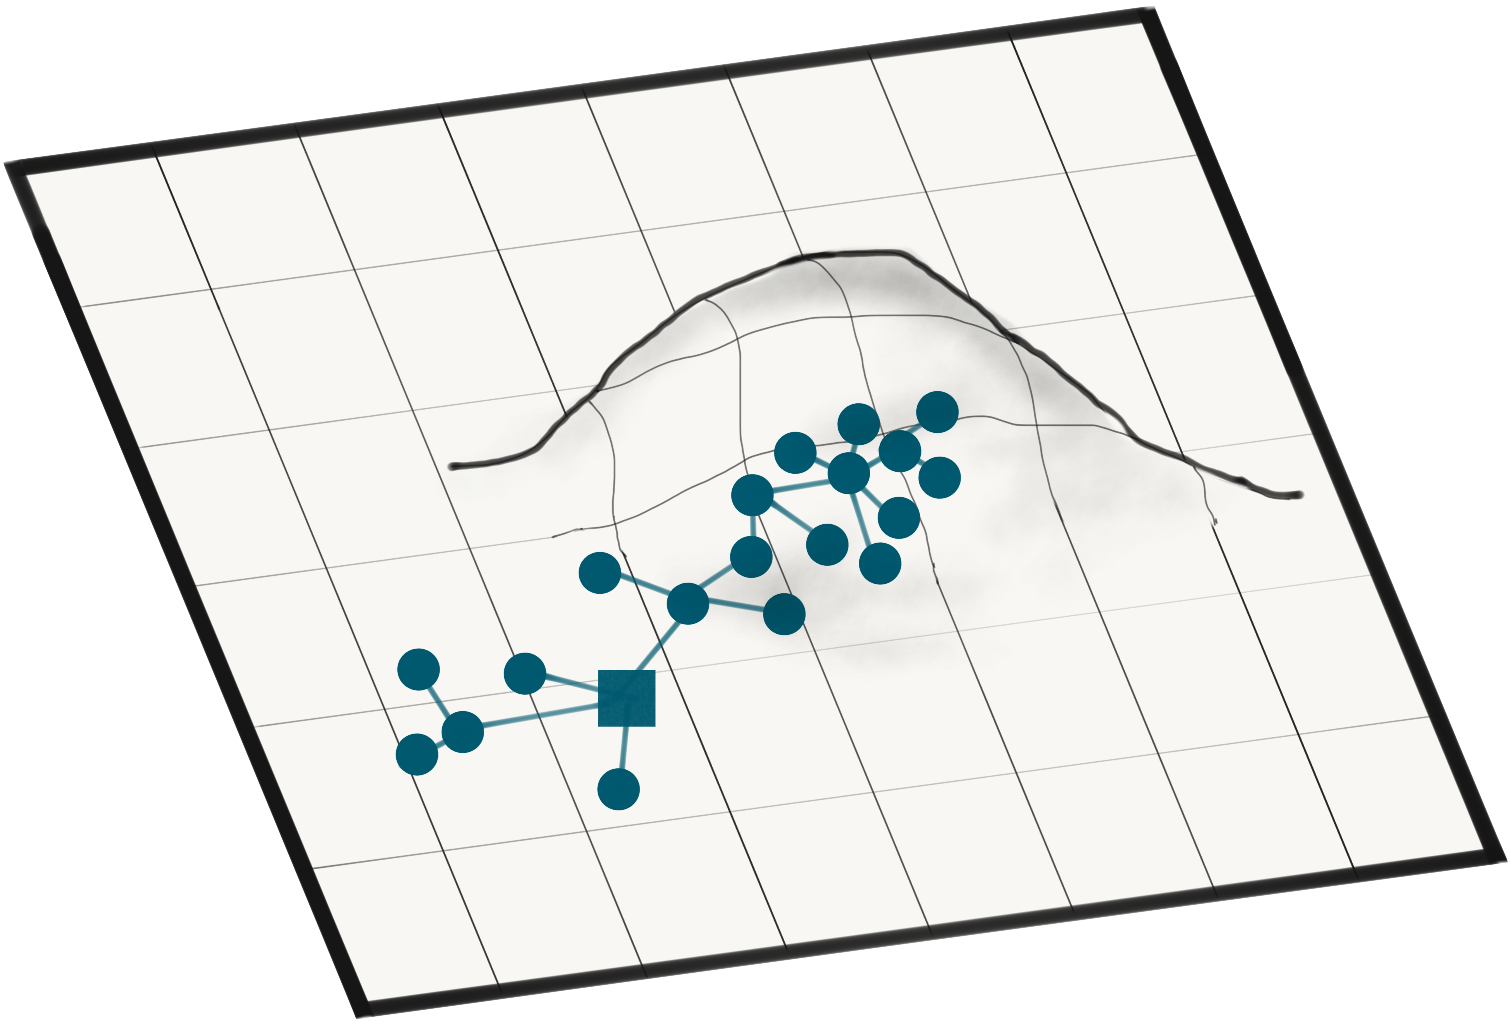
\includegraphics[width=\textwidth]{img/fast_cooling.png}
        \caption{fast cooling rate}
        \label{subfig:fast_cooling}
    \end{subfigure}
 	\captionsetup{singlelinecheck=off,justification=raggedright}
    \vspace{-2ex}
  \captionsetup{singlelinecheck=off,justification=raggedright}
  \caption{The three modes of local phenotype space search proposed are illustrated. In each illustration, the phenotype space is depicted as a three dimensional surface with points on the surface representing different phenotypes and the height of the surface denoting the fitness of the phenotypes at those points. The original phenotype mapped to by a genetic representation is shown with a square. Points marked with a circle denote phenotypes explored during the local search processes. Lines connecting the points represent that one point was reached from the other by a mutation of the direct representation of a phenotype. Subfigure \ref{subfig:static_mutation} depicts the direct mutation local phenotypic search process, where points explored are generated by mutations to the direct representation of the original phenotype mapped to by a genetic representation. Subfigure \ref{subfig:random_walk} depicts the random walk local phenotypic search process, where points explored are generated by mutation to the direct representation of the point explored immediately before (starting from the direct representation of the original phenotype mapped to by a genetic representation). Finally, subfigure \ref{subfig:simulated_annealing} depicts the simulated annealing local phenotypic search process, where points are explored via mutation to the direct representation of a randomly chosen point previously explored with an increasingly strong bias towards exploring from points with high fitness as the exploration process proceeds.}
  \label{fig:local_search_types}
\end{figure}